% 02.06.2016 12:00 CET last changed by a.holzinger
% General Template for LNCS and LNAI contributions based on llncs, adapted by ah
% Many thanks to the TRS team
% In case of using eps compile via 1) TeXify and then proceed with 2) dvi2pdf
%
\documentclass{llncs}

\usepackage[dvips]{graphicx}
\usepackage[ruled,vlined]{algorithm2e}
\usepackage{amsfonts}
\usepackage{amssymb}
\usepackage{amsmath}
\usepackage{mathtools}

\providecommand{\abs}[1]{\lvert#1\rvert}
\providecommand{\norm}[1]{\lVert#1\rVert}

\usepackage{calc}
\usepackage{subfigure}

\usepackage{color}
\usepackage{soul}
\usepackage{comment}

\newtheorem{prop}{Property}

\newenvironment{Bitemize}{\renewcommand\labelitemi{\textbullet}\begin{itemize}}{\end{itemize}}

\begin{document}

\title{Toward Machine Learning on perturbed knowledge baes}

\author{Bernd Malle, Peter Kieseberg, Edgar Weippl, Andreas Holzinger}
\institute{Holzinger Group HCI-KDD \\
Institute for Medical Informatics, Statistics \& Documentation\\
            Medical University Graz, Austria\\
            \texttt{b.malle@hci-kdd.org}}

\maketitle

\begin{abstract}
	
The amount of patient-related data produced in today’s clinical setting poses many challenges with respect to collection, storage and responsible use. For example, in research and public health care analysis, data must be anonymized before transfer, for which the k-anonymity measure was introduced and successively enhanced by further criteria. As k-anonymity is an NP-hard problem, modern approaches often make use of heuristics based methods. This paper will convey the motivation for anonymization followed by an outline of its criteria as well as a general overview of methods \& algorithmic approaches to tackle the problem. \\

As the resulting data set will represent a trade-off between utility and individual privacy, we need to optimize those measures to individual (subjective) standards. Moreover, the efficacy of an algorithm strongly depends on the background knowledge of a potential attacker as well as the underlying problem domain. Therefore, it seems logical to adapt the process including expert domain knowledge, which can be done via an interactive machine learning (iML) approach. We will therefore point out how domain experts might get involved to improve upon current methods and introduce an example setup based on the SaNGreeA algorithm; due to this algorithm's nature of taking into account structural (network) as well as information properties of the underlying problem domain, it can be useful for (but also limited to) common tabular data anonymization. \\

We will present our work by demonstrating a Web-based User Interface to conduct interactive machine learning tasks and compare the results of a variety of different parameter settings from our iML experiments with a standard industry anonymization algorithm in terms of efficiency, information loss as well as threat scenarios \hl{No idea how to do that yet...}. A discussion of future developments and possibilities will finally conclude this paper.


\medskip

\textbf{Keywords}: machine learning, interactive machine mearning, anonymization, k-anonymity, SaNGreeA, information loss, structural loss, cost weighing vector


\end{abstract}

\renewcommand{\thesubfigure}{\thefigure.\arabic{subfigure}}
\makeatletter
\renewcommand{\p@subfigure}{}
\renewcommand{\@thesubfigure}{\thesubfigure:\hskip\subfiglabelskip}
\makeatother

\section{Introduction and Motivation for Research}

Privacy preserving machine learning is an important issue, fostered by anonymization \cite{Samarati:2001:kAnonymity}, in which a record is released only if it is indistinguishable from $k$ other entities in the data. k-anonymity is highly dependent on spatial locality in order to effectively implement the technique in a statistically robust way, and in high dimensionalities data becomes sparse, hence, the concept of spatial locality is not easy to define. Consequently, it becomes difficult to anonymize the data without an unacceptably high amount of information loss \cite{Aggarwal:2005:kAnonymity}. Consequently, the problem of k-anonymization is on the one hand NP-hard, on the other hand the quality of the result obtained can be measured at the given factors: \emph{k-anonymity} means that attributes are suppressed or generalized until each row in a database is identical with at least $k-1$ other rows   \cite{Sweeney:2002:k-Anonymity}; \emph{l-diversity} as extension of the k-anonymity model reduces the granularity of data representation by generalization and suppression so that any given record maps onto at least $k$ other records in the data \cite{MachanavajjhalaEtAl:2007:l-Diversity}; \emph{t-closeness} is a refinement of l-diversity by reducing the granularity of a data representation, and treating the values of an attribute distinctly by taking into account the distribution of data values for that attribute \cite{LiEtAl:2007:t-closeness}; and \emph{delta-presence}, which links the quality of anonymization to the risk posed by inadequate anonymization \cite{NergizClifton:2010:Delta-Presence}, but not with regard to the actual security of the data, i.e., the re-identification through an attacker. For this purpose certain assumptions about the background knowledge of the hypothetical enemy must be made. With regard to the particular demographic and cultural clinical environment this is best done by a human agent. Thus, the problem of (k-)anonymization represents a natural application domain for iML \cite{Holzinger:2016:iML}, \cite{Kieseberg:2016:Doctor-in-the-Loop}.

\begin {comment}
\section{Glossary and Key Terms}
NOTE: this section may not to be used for a conference
\textbf{Note: This is only for use when producing a Springer LNCS SOTA State-of-the-Art-Analysis paper}
\\[0,2cm]
\emph{SaNGreeA} is the abbreviation for Social Network Greedy Anonymization, which describes an anonymization algorithm which takes into account information loss as well as structural loss (from anonymizing the neighborhood of a network node). It is said to be greedy as it uses greedy clustering under the hood in order to avoid having to sift through an exponential solution space to find an optimum.

\end{comment}

\section{Basic Concepts}
\label{sect:basic_concepts}

\subsection{Tabular anonymization}
\label{ssect:tab_anonym}

Taking a look at Figure~\ref{fig:anon_categories} will help the reader in understanding the original (tabular) concept of anonymization: Given an input table with several columns, we will probably encounter three different categories of data:

\begin{itemize}
	\item \textbf{Personal identifiers} are data items which directly identify a person without having to cross-reference or further analyze them. Examples are first and last names, but even more so an (email) address or social security number (SSN). As personal identifiers are dangerous and cannot be generalized (see Figure~\ref{fig:gen_hierarchy}) in a meaningful way (e.g. one could generalize the \textit{address} field, which would only result in some kind of Zip code), this category of data is usually removed. The table shows this column in a red background color.
	\item \textbf{Sensitive data,} also called 'payload', which is the kind of data we want to convey for statistics or research purposes. Examples for this category would be disease classification, drug intake or personal income level. This data shall be preserved in the anonymized dataset and can therefore not be deleted or generalized. The table shows this column in a green background color.
	\item \textbf{Quasi identifiers}, colored in the table with an orange background, are data that in themselves do not directly reveal the identity of a person, but might be used in aggregate to reconstruct it. For instance, \cite{sweeney2002k} mentioned that 87\% of U.S. citizens in 2002 had reported characteristics that made them vulnerable to identification based on just the 3 attributes \textit{zip code}, \textit{gender} and \textit{date of birth}. But although this data can be harmful in that respect, it might also hold vital information for the purpose of research (e.g. zip code could be of high value in a study on disease spread). The solution - and this is the actual point of all anonymization efforts - is to generalize this kind of information, which means to lower its level of granularity. As an example, one could generalize the ZIP codes 41074, 41075 and 41099 to a generalized version 410**, as shown in Figure~\ref{fig:anonymized_clusters}.
\end{itemize}

\begin{figure}[!t]
	\begin{center}
		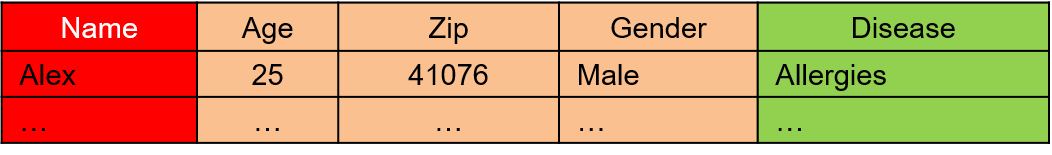
\includegraphics[width=0.9\textwidth]{figures/anonym/3typesofdata}
		\caption{The three types of data considered in (k-)anonymization}
		\label{fig:anon_categories}
	\end{center}
\end{figure}

As described in \cite{ciriani2007kappa}, k-anonymization requires that in each data release every combination of values of quasi-identifiers must be identical to at least $k-1$ other entries in that release, which can be seen as a clustering problem with each cluster's (in the context of anonymization also called an 'equivalence class') internal quasi-identifier state being identical for every data point. This can be achieved via suppression and generalization, where suppression means simply deletion, whereas in generalization we try to retain some usable value.

The process of generalization works through a concept called \textit{generalization hierarchies}, which form a tree whose root denotes the most general value available for a data category (usually the 'all' value) and then branches to more and more specific occurrences, with its leafs representing the set of exact, original values (see Figure~\ref{fig:gen_hierarchy}). In generalizing some original input value, one traverses the tree from the leaf level upwards until a certain prerequisite is fulfilled. Usually, this prerequisite comes in the form of the k-anonymity requirement, so that we want to find a group of other data rows (=vectors) whose (generalized) quasi identifiers match the data point being processed.

\begin{figure}[!t]
	\begin{center}
		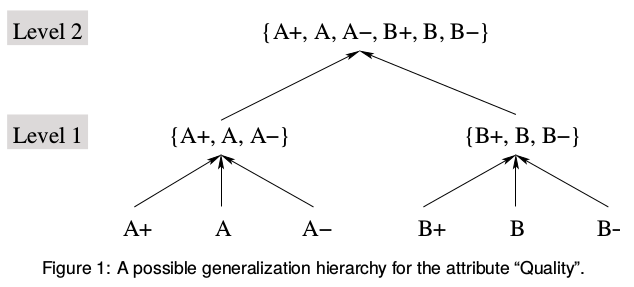
\includegraphics[width=0.8\textwidth]{figures/anonym/gen_hierarchy}
		\caption{Example of a typical generalization hierarchy}
		\label{fig:gen_hierarchy}
		\small
		taken from \cite{aggarwal2005approximation}
	\end{center}
\end{figure}


Each level of generalization involves a certain cost in information loss though, which means we do not just want to construct our clusters in any sequence possible, but minimize the overall information loss. This makes k-anonymization an NP-hard optimization problem (because of an exponential number of possible generalized quasi-identifier combinations), leaving us to conclude that the k-Anonymity problem is to lose as little information as possible in a dataset while ensuring that the release (the anonymized, publishable version of the dataset) satisfies the k-anonymization criterion \cite{aggarwal2005approximation}.

\begin{figure}[!t]
	\centering
	\begin{minipage}[b]{0.5\textwidth}
		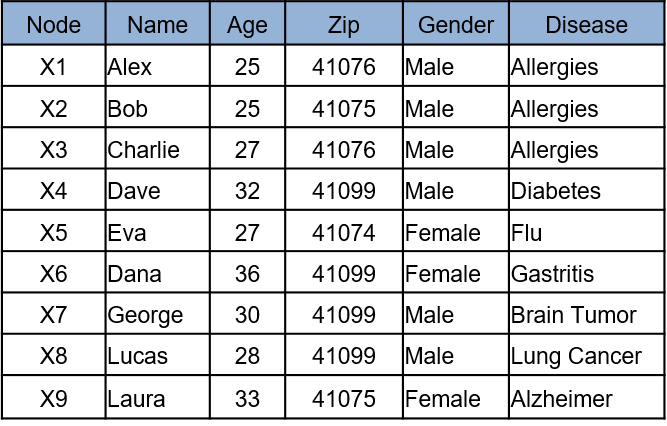
\includegraphics[width=\textwidth]{figures/anonym/k_anon_input}
	\end{minipage}
	\hfill
	\begin{minipage}[b]{0.418\textwidth}
		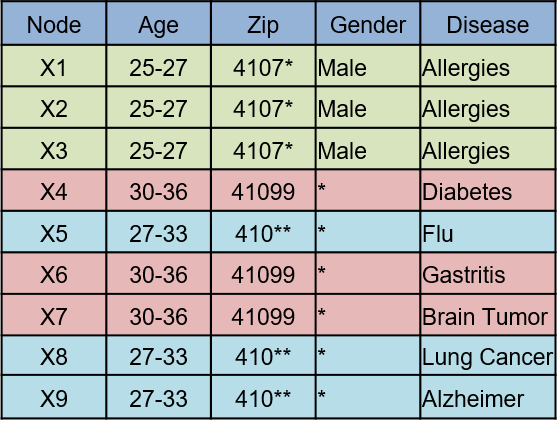
\includegraphics[width=\textwidth]{figures/anonym/k_anon_output}
	\end{minipage}
	\caption{Tabular anonymization: input table and anonymization result}
	\label{fig:anonymized_clusters}
\end{figure}


\subsection{Graph (social network) anonymization}
\label{ssect:graph_sn_anon}

In the last section we were solely concerned with tabular data; However, as social networks have gained huge popularity over the previous decade, and even modern medical databases come in the form of graph structures, the question of how to efficiently anonymize networks has gained ever more significance over the years.

As a start, one could see a graph just as a collection of nodes, where each node contains some kind of feature vector, akin to the row in a data table. Adopting that view, we could be tempted to simply ignore the existence of edges and apply some kind of algorithm suitable to the anonymization of tabular data. The main problem with this however lies in the fact that the structural environment of a node (the constellation of its neighbors within the greater network) provides some additional information. That is, even if we successfully (k-)anonymize the feature vectors of a graph according to the methods found in the previous chapter, we still run the risk of leaving to much information in the form of a known local subgraph structure.

Consider Figure~\ref{fig:anon_sn_problem} for example, in which the nodes of a graph have already been k-anonymized into groups of size 3 and 7, respectively. In this figure, local subgraphs b) and c) are actually (3)-anonymized, because as each node has the exact same local neighborhood structure, the additional information of a node possessing a degree of 0 (or 2) is of no additional value. For local subgraphs a) and d) on the other hand, the additional information of a node being of degree (x) has the potential to reveal its identity, as it is not indistinguishable from its neighbors within the equivalence class any more.

\begin{figure}[!t]
	\begin{center}
		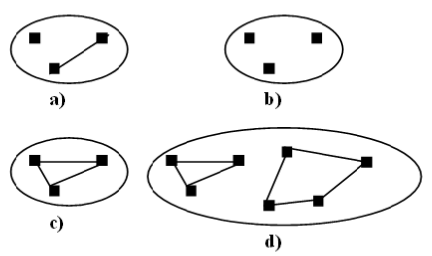
\includegraphics[width=0.8\textwidth]{figures/anonym/sn_problem}
		\caption{Local subgraph neighborhoods as additional anonymization obstacle.}
		\label{fig:anon_sn_problem}
	\end{center}
	\small
	(Example taken from \cite{campan2009data}.)
\end{figure}


\section{Related work}
\label{sect:related_work}


Several methods have been proposed to make re-identification of nodes in anonymized social graphs harder.	\cite{chester2011k} for example introduce the idea of vertex addition to labeled and unlabeled datasets. While an algorithm on the former remains NP complete, they provide an efficient ($O(nk)$) algorithm for unlabeled data. Experimenting on several well known datasets, they show that commonly-studied structural properties of the network, such as clustering coefficient, are only minorly distorted by their anonymization procedure.

The authors of \cite{kapron2011social} take the approach of adding edges to an edge-labeled graph like the Netflix movie database (with users and movies being nodes and edge weights representing movie ratings). They define tables as bipartite graphs and prove NP-hardness for the problems of neighborhood anonymity, i-hop anonymity and k-symmetry anonymity.

\cite{campan2009data}, whose local subgraph problem we already encountered, proposed a solution in the form of a greedy clustering algorithm which takes into account not only the information loss incurred by generalizing features of nodes, but also introducing a structural loss function based on the local neighborhood within an equivalence class (and between them). The author of this thesis implemented that approach utilizing GraphiniusJS and will demonstrate the algorithm in Section~\ref{sect:aoa_anonymization} as well as the anonymized results in Appendix Section~\ref{sect:anon_output_data}.


\section{Experiments}
\label{sect:experiments}


\subsection{Data} 
\label{ssect:data}


\subsection{Experiments}
\label{ssect:experiments}


\subsection{Algorithm}
\label{ssect:algorithm}


SaNGreeA stands for \textit{Social network greedy clustering} and was introduced by \cite{campan2009data}. In addition to 'clustering' nodes of a graph according to the minimum general information loss (GIL) incurred as described in Section~\ref{sect:graph_sn_anon}, this algorithm also considers the structural information loss (SIL) by assigning a node to a certain cluster. The SIL quantifies the probability of error when trying to reconstruct the structure of the initial graph from its anonymized version.

The SIL is composed of two different components: 1) the intra-cluster structural loss, signifying the error probability in trying to reconstruct the original edge distribution within an equivalence class (= anonymized cluster), and 2) the inter-cluster structural loss which represents the error probability in trying to reconstruct the original configuration of edges between two equivalence classes.

In implementing and demonstrating this algorithm, I recreated the paper's original experiment:

\begin{enumerate}
	\item \textbf{Process input data into suitable structure.} The adults dataset was selected and all but six columns deleted - only Age, Workclass, Country of origin, Gender, Race and Marital status remained (a sample containing the first 19 rows can be seen in Figure~\ref{fig:adult_input_data_sample}). Furthermore, in order to obtain repeatable results, the first 300 'pure' rows (no missing or mis-formatted values) in the dataset were chosen as input set.
	
	\item \textbf{Enhance structure with graph information (random edges).} Using GraphiniusJS's capability of randomly adding edges to nodes, a connected graph was created out of the assortment of nodes (using between 1 and 10 outgoing edges per node).
	
	\item \textbf{Compute GIL \& NGIL.} The general information loss with respect to a cluster is given by the following formula (repeating from the original paper):
	\begin{equation*}
	\text{GIL}(cl) = \abs{cl} \cdot (\sum_{j=1}^{s} \frac{size(gen(cl)[N_j])}{size(min_{x \epsilon N} (X[N_j]), max_{x \epsilon N} (X[N_j]))} + \sum_{j=1}^{t} \frac{height(\Lambda(gen(cl)[C_j]))}{height(H_{C_j})})
	\end{equation*}
	where:\\
	- $\abs{cl}$ denotes the cluster cl's cardinality; \\
	- $size([i1,i2])$ is the size of the interval $[i1,i2]$, i.e., $(i2-i1)$; \\
	- $\Lambda(w), w \epsilon H_{C_j}$ is the subhierarchy of $H_{C_j}$ rooted in $w$; \\
	- $height(H_{C_j})$ denotes the height of the tree hierarchy $H_{C_j}$; \\
	
	The total generalization information loss is then given by:
	\begin{equation*}
	\text{GIL}(G,S) = \sum_{j=1}^{v} \text{GIL}(cl_j)
	\end{equation*}
	And the normalized generalization information loss by:
	\begin{equation*}
	\text{NGIL}(G,S) = \frac{\text{GIL}(G,S)}{n \cdot (s+t)}
	\end{equation*}
	
	\item \textbf{Compute SIL \& NSIL.} For the exact mathematical definitions of SIL \& NSIL the reader is kindly referred to the original paper. Because the structural information loss cannot be computed exactly before the final construction of clusters, the exact computations were replaced by the following distance measures: \\
	Distance between two nodes:
	\begin{equation*}
	\text{dist}(X^i, X^j) = \frac{\abs{\{l|l=1..n \wedge l \ne i,j;b_l^i \ne b_l^j}}{n-2}
	\end{equation*}
	
	Distance between a node and a cluster:
	\begin{equation*}
	\text{dist}(X, cl) = \frac{\sum_{X^j \epsilon cl} \text{dist}(X, X^j) }{\abs{cl}}
	\end{equation*}
\end{enumerate}

The algorithm starts with initializing a first cluster by simply adding a randomly chosen node to it. Then, for every new node encountered, the weighted sum of the above two information loss metrics will yield a certain overall information loss value if the node was added to that cluster - the node with the minimal cost is then chosen as the candidate and expands the cluster. This is repeated until the first cluster reaches a certain requirement (e.g. size $ \coloneqq  k $ -factor) upon which another random node is chosen to constitute a next cluster. This procedure is repeated until all nodes have been assigned (if a cluster of size < k-factor remains, its member nodes are dispersed amongst the others). 

Since the algorithm does not take ALL possible node combinations into account, but simply start with a node and compares all the candidates in a loop, the algorithm runs in quadratic time w.r.t. the input size in number of nodes. This worked well within milliseconds for an input problem size of a few hundred nodes. An example output of the implemented algorithm can be found at \hl{Enter Graphinius URL here}. \\


\begin{figure}[!t]
	\begin{center}
		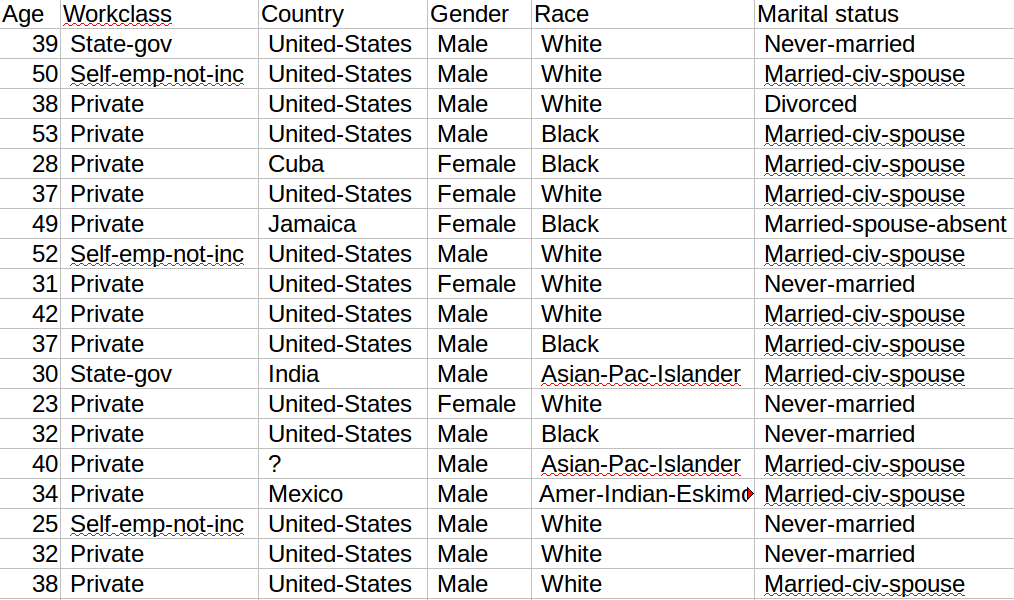
\includegraphics[width=1\textwidth]{figures/anonym/anon_adults_input_sample_pic}
		\caption{Excerpt: the first 25 rows of the Adult census data set}
		\label{fig:adult_input_data_sample}
	\end{center}
\end{figure}


\section{Results}
\label{sect:results}


\section{Discussion}
\label{sect:discussion}


\section{Open problems and future challenges}
\label{sect:op_fc}


\section{Conclusion}
\label{sect:conclusion}



\newpage

\bibliographystyle{plain}
\bibliography{references}

\end{document}










\begin{comment}
At the beginning provide a motivation on why your paper is interesting. Example:
ML is very broad and deals with the problem of extracting features from data to solve predictive tasks, including decision support, forecasting, ranking, classifying (e.g., in cancer diagnosis), detecting anomalies (e.g., virus mutations) or sentiment analysis \cite{PetzEtAl:2015:Sentiment}. The challenge is to discover relevant \emph{structural} patterns and/or \emph{temporal} patterns (``knowledge") in such data, which are often hidden and not accessible to the human expert. The problem is that a majority of the data sets in the biomedical domain are weakly-structured and non-standardized \cite{HolzingerEtAl:2014:KDDBio}, and most data is in dimensions much higher than $3$, and despite human experts are excellent in pattern recognition for dimensions $\leq 3$, such data make manual analysis often impossible.

Most colleagues from the ML community are concentrating on \textit{automatic} machine learning (aML), with the grand goal of bringing humans-out-of-the-loop, and a best practice real-world example can be found in autonomous vehicles.

However, biomedical data sets are full of uncertainty, incompleteness etc. \cite{Holzinger:2014:SpringerTextbook}, they can contain missing data, noisy data, dirty data, unwanted data, and most of all, some problems in the medical domain are hard, which makes the application of fully automated approaches difficult or even impossible, or at least the quality of results from automatic approaches might be questionable. Moreover, the complexity of sophisticated machine learning algorithms has detained non-experts from the application of such solutions.
Consequently, the integration of the knowledge of a domain expert can sometimes be indispensable and the interaction of a domain expert with the data would greatly enhance the knowledge discovery process pipeline.
Hence, \textit{interactive} machine learning (iML) puts the ``human-in-the-loop" to enable what neither a human nor a computer could do on their own. This idea is supported by a synergistic combination of methodologies of two areas that offer ideal conditions towards unraveling such problems: Human-Computer Interaction (HCI) and Knowledge Discovery/Data Mining (KDD), with the goal of supporting human intelligence with machine intelligence to discover novel, previously unknown insights into data (HCI-KDD approach \cite{Holzinger:2013:HCI-KDD}).

\textbf{We define iML-approaches as algorithms that can interact with \textit{both computational agents and human agents} *) and can optimize their learning behaviour through these interactions.} \cite{Holzinger:2016:iML}

*) In Active Learning such agents are referred to as so-called ``oracles".

This template is based on the TRS: The {\it Transactions on Rough Sets} ({\em TRS} journal is an outgrowth of the pioneering work on rough sets by Zdzis{\l}aw Pawlak (see, {\em e.g.},~\cite{rs0,rs1,rs2,rs3,objects,RS}) and many others~\cite{RSDS} during the past three decades.

This Styleguide for preparing an article for submission to the TRS has the following organization:  The \LaTeX~document class to be used by every author is specified in Sect.~\ref{req}.  In addition, information about \LaTeX~as well as information about public domain software for \LaTeX~users is also given in Sect.~\ref{req}.  A very detailed set of style guidelines that must be used in preparing an article for the TRS can be found in Sect. [style].  Notice that this document illustrates how each of the article components described in the Style Guideline can be performed in \LaTeX.  In effect, this document can be used as a template for a TRS article. The method of submission of an article to the TRS is given in Sect. [method]. Finally, the specification for the concluding section of a TRS article is given in Sect.~\ref{summary}.
% ~\ref{method}
% ~\ref{style}


\section{\LaTeX~Requirements}\label{req}
Prepare your TRS paper using {\bf \LaTeX} and the Springer-Verlag document class llncs.cls (see ~\cite{springer}).  There are a number of books that are helpful in showing how to use \LaTeX~(see, {\em e.g.},~\cite{math,graphics,companion}).  A tutorial to help you get started in preparing a~\LaTeX~document is available at~\cite{tutorial}.  To find the latest version of~\LaTeX, try~\cite{latest}. Articles written in Microsoft \textregistered~Word will not be accepted.

MiKTeX (pronounced mik-tech) is an up-to-date implementation of \TeX~\cite{texmanual}, which is available for different platforms\footnote{See $http://www.tex.ac.uk/cgi-bin/texfaq2html?label=TeXsystems$.}.  For example, \TeX\ and related programs is available for Windows on a PC (all current variants), MacOS X, Linux, and Unix. \TeX\ is a typesetting system invented by D.E. Knuth~\cite{knuth05}, who has written that~\LaTeX~is ``intended for the creation of beautiful books--and especially for books that contain a lot mathematics''.  More information about \TeX\ (its history, novel aspects of \TeX, examples, software, notes, references as well as external links) can be found at~\cite{tex}. The MiKTeX system is public domain software that is available from~\cite{miktex}.  The \verb|graphicx|, \verb|algorithm2e|, and \verb|subfigure| packages used in this document, are among the files that can be downloaded from the web (see, {\em e.g.},~\cite{alg2e,graph,subfig}).

It is also important to have access to a \LaTeX~editor such as TeXnicCenter, which is an Integrated Development Environment for writing TeX/LaTeX-documents on Microsoft Windows \textregistered~platforms\cite{texnic}.    TeXnicCenter provides a lot of enhanced features like structure parsing, project management, syntax highlighting, and so on.  TeXnicCenter is also public domain software available from~\cite{texcenter}.

\section*{Symbols in~\LaTeX}
\label{symb}

A comprehensive list of 3300 symbols commonly available to~\LaTeX~users as well as the corresponding~\LaTeX~commands used to produce the symbols is available from~\cite{symbols}.  Tables \ref{lg}-\ref{relation} present some of the more commonly used symbols in \LaTeX.

\begin{table}
\begin{center}
\caption{\label{lg}Lowercase Greek Letters}
\renewcommand{\arraystretch}{0.5}
\setlength\tabcolsep{3pt}
\begin{tabular}{llllllll}
\hline\noalign{\smallskip}
$\alpha$ 			& $\backslash$alpha 			& $\theta$ 	& $\backslash$theta	 & $o$ 	  & $\backslash$o & $\tau$ 	& $\backslash$tau\\
$\beta$ 			& $\backslash$beta 				& $\vartheta$ & $\backslash$vartheta & $\pi$ & $\backslash$pi & $\upsilon$ 	& $\backslash$upsilon\\
$\gamma$ 			& $\backslash$gamma 			& $\iota$   & $\backslash$iota   & $\varpi$     & $\backslash$varpi & $\phi$ 	& $\backslash$phi\\
$\delta$ 			& $\backslash$delta 			& $\kappa$ 	& $\backslash$kappa	 & $\rho$ & $\backslash$rho & $\varphi$ 	& $\backslash$varphi\\
$\epsilon$ 		& $\backslash$epsilon 		& $\lambda$ & $\backslash$lambda & $\varrho$    & $\backslash$varho & $\chi$ 	& $\backslash$chi\\
$\varepsilon$ & $\backslash$varepsilon 	& $\mu$ 		& $\backslash$mu 		 & $\sigma$     & $\backslash$sigma & $\psi$ 	& $\backslash$psi	 \\
$\zeta$ 			& $\backslash$zeta 				& $\nu$ 		& $\backslash$nu 		& $\varsigma$& $\backslash$varsigma & $\omega$ 	& $\backslash$omega	 \\
$\eta$ 				& $\backslash$eta 				& $\xi$ 		& $\backslash$xi\\
\hline
\end{tabular}
\end{center}
\end{table}

\vspace{-10mm}

\begin{table}
\begin{center}
\caption{\label{cg}Uppercase Greek Letters}
\renewcommand{\arraystretch}{0.5}
\setlength\tabcolsep{3pt}
\begin{tabular}{llllllll}
\hline\noalign{\smallskip}
$\Gamma$ & $\backslash$Gamma & $\Lambda$ & $\backslash$Lambda & $\Sigma$ & $\backslash$Sigma & $\Psi$ & $\backslash$Psi\\
$\Delta$ & $\backslash$Delta& $\Xi$ & $\backslash$Xi& $\Upsilon$ & $\backslash$Upsilon& $\Omega$ & $\backslash$Omega\\
$\Theta$ & $\backslash$Theta& $\Pi$ & $\backslash$Pi& $\Phi$ & $\backslash$Phi\\
\hline
\end{tabular}
\end{center}
\end{table}

\vspace{-10mm}

\begin{table}
\begin{center}
\caption{\label{relation}Relation Symbols}
\renewcommand{\arraystretch}{0.5}
\setlength\tabcolsep{3pt}
\begin{tabular}{llllllll}
\hline\noalign{\smallskip}
$\in$ & $\backslash$in & $\notin$ & $\backslash$notin & $\cap$ & $\backslash$cap & $\cup$ & $\backslash$cup\\
$\approx$ & $\backslash$approx & $\rightarrow$ & $\backslash$rightarrow & $\prec$ & $\backslash$prec & $\subset$& $\backslash$subset\\
$\asymp$ & $\backslash$asymp & $\Join$ & $\backslash$Join & $\preceq$ & $\backslash$preceq & $\subseteq$& $\backslash$subseteq\\
$\bowtie$ & $\backslash$bowtie & $\leq$ & $\backslash$leq & $\propto$ & $\backslash$proto & $\succ$& $\backslash$succ\\
$\cong$ & $\backslash$cong & $\ll$ & $\backslash$ll & $\sim$ & $\backslash$sim & $\succeq$& $\backslash$succeq\\
$\dashv$ & $\backslash$dashv & $\mid$ & $\backslash$mid & $\simeq$ & $\backslash$simeq & $\supset$& $\backslash$supset\\
$\doteq$ & $\backslash$doteq & $\models$ & $\backslash$models & $\smile$ & $\backslash$smile & $\supseteq$& $\backslash$supseteq\\
$\equiv$ & $\backslash$equiv & $\neq$ & $\backslash$neq & $\vdash$ & $\backslash$vdash & $\forall$ & $\backslash$forall\\
$\gg$ & $\backslash$gg & $\ni$ & $\backslash$ni  & $\frown$ & $\backslash$frown & $\perp$ & $\backslash$perp\\
$\geq$ & $\backslash$geq & $\parallel$ & $\backslash$parallel & $\exists$ &$\backslash$exists & $\emptyset$ & $\backslash$emptyset\\
\hline
\end{tabular}
\end{center}
\end{table}

\vspace{-8mm}

\subsection{Abstract}
The abstract for your article should briefly describe the problem(s) solved in your article.  Include in your description, a brief indication of the context for your research.  Then indicate if you have included such things as examples, sample experimental results, and data.  Finally, clearly state the contribution of your article.  Abstracts are usually between 100 and 150 words in length (longer abstracts are also acceptable).

\subsection{Keywords}
A {\it keyword} is a significant or descriptive word that helps identify a focal point in the subject matter ({\em i.e.}, principal topic) of a research article.  Keywords provide a basis for searches for published articles on a particular subject, and have been the subject of considerable research (see, {\em e.g.},~\cite{keywords}).
After your Abstract in a TRS article, give a list of up to 8 keywords or phrases that indicate the principal topics covered in your article.

\subsection{Introduction}
The Transactions on Rough Sets (TRS) is the primary publication of the International Rough Set Society (IRSS~\cite{IRSS}).   Your article should begin with a thorough introduction.  This Introduction should begin by clearly describing the problem(s) to be solved in your article.  The description of the problem should be followed by an indication of the approach to solving the problem in your article.  The problem-description should include a carefully crafted overview of the context for the problem.  This context must include references to the principal (and, possibly, minor) works that are currently published on this subject (see, {\em e.g.},~\cite{RSDS} for a comprehensive list of papers on rough sets and their applications).  After giving a description of the problem(s) solved in your article, clearly indicate the contribution(s) of your article.  In doing this, you should compare and contrast your contribution(s) with related contributions in papers published by others.  Finally, your introduction should conclude with an overview of the organization of your article.

\subsection{Basic Concepts}  After your introduction, introduce a section that gives an overview of the basic concepts that underly the contribution(s) of your article.  This Basic Concepts section should be sufficiently detailed so that the connection between traditional basic concepts and notation and the new results presented by you in succeeding sections of your article, is made clear.  Document the sources of the concepts and notation that you introduce in this Basic Concepts section.

\subsection{Details} Include sections (and subsections) that give further details about the research introduced in the article.  Such sections should make it clear what is intended by the research presented in the article.  This can be accomplished by first giving a detailed presentation of notation, data, experiments, algorithms, and theory related to what you present.  After that, compare and contrast the results and methods presented in your article with results and methods presented by other researchers.  This means that you must document the claims made in your article, and give a complete presentation of results found in works related to your research.  By doing this, you will provide the reader with a clearcut view of your research and its context.

\subsection{Notation} As an aid to understanding the intricacies of the research contribution presented in your article, be sure to introduce, explain, and document the notation that you use.  It is preferable to use notation traditionally employed in rough set theory rather than using new notation that is equivalent to the common notation.  In other words, the following rule-of-thumb should be followed: {\it be conservative in the introduction of new notation in connection with your research}.  Otherwise, it becomes very difficult for reviewers to follow what you are writing.  If you find it necessary to introduce new notation, then it should be clearly explained, illustrated, and distinguished from existing notation.

\subsection{Data} Include sections (and subsections) that give a detailed description of the data used to obtain experimental results.  This description should include sample data and an indication of the sources of your data.  It will be very good if the data used in your article is made available either at~\cite{IRSS} or at some other website.

\subsection{Experiments} Include sections (and subsections) that give a detailed presentation of experimental results used in support of the claims made in your paper.   It is recommended that a presentation of the experimental results include carefully labeled plots, charts, and tables.  Document your experimental results by comparing and contrasting them to results obtained by other researchers.

\begin{algorithm}[!t]
 \caption{Off-Policy Monte Carlo Control Algorithm\label{MCoff}}
 \DontPrintSemicolon

 \SetKwData{Left}{left}
 \SetKwData{This}{this}
 \SetKwData{Up}{up}
 \SetKwFunction{Union}{Union}
 \SetKwFunction{FindCompress}{FindCompress}
 \SetKwInOut{Input}{Input}
 \SetKwInOut{Output}{Output}

\Input{States $s\in \textsl{S} $,~Actions~$ a\in A(s)$ //$A(s)$ is a set of actions in state \emph{s}.}
\Output{Policy $\pi(s)$ //where $\pi(s)$ is a policy in state $s$ that controls the selection of a particular action in state $s$.}

 \SetAlgoLined
 \For{$\left( all ~s\in \textsl{S}, a\in A(s)\right)$}
  {$\pi(s)$ is randomly chosen;\\
  $Q\left(s,a\right)  \longleftarrow $ arbitrary; //where $Q$ is the value of an action $a$ is state $s$\;
   $N(s,a)  \longleftarrow  0 ; \quad $//numerator~of~$Q(s,a)$ \;
   $D(s,a)  \longleftarrow  0 ; \quad $//denominator~of~$Q(s,a)$ \;
  }%ebd for
\While{True}
{Select an action policy $ \pi'(s,a)$, and use it to generate an episode: $$s_0,a_0,r_1,s_1,a_1,r_2,\ldots,s_{T-1},a_{T-1},r_T,s_T; \mbox{ // } r_i \mbox{ is the reward on action } a_{i-1}$$\;
$\tau \longleftarrow \mbox{ the latest time at which } a_{\tau} \neq \pi(s_{\tau})$;\;

 \For{each pair $\left(s,a\right)$ appearing in the episode at time $ \tau$  or later} {
 $t \longleftarrow \mbox{ the time of first occurrence of } s,a \mbox{ such that } t\geq \tau$; \;
 $w  \longleftarrow \prod_{k=t+1}^{T-1} \frac{{1}}{\pi^{\prime}(s_k,a_k)};$  // weight on $R_t=\sum_{i=t+1}^{T}r_{i}$;
  $N(s,a)  \longleftarrow N(s,a) + wR_t  $; \;
  $D(s,a)  \longleftarrow D(s,a) + w $; \;
  $Q(s,a)  \longleftarrow \frac{{N(s,a)}}{{D(s,a)}} ; $\;
  }%end for
 \For{each $ \textsl{s} \in S $}
  {$ \pi (s) \longleftarrow   argmax_a   Q(s,a)$; \;
  }%end for
 } %end While

\end{algorithm}

\subsection{Algorithms} Include detailed algorithms that specify the steps used in the research presented in the article.  Each algorithm should be accompanied by an explanation of the principal steps, and the significance of the notation used in the algorithm.  Document your algorithms by comparing and contrasting them with methods used by other researchers.  Consider, for example, the reinforcement learning algorithm given in Alg.~\ref{MCoff}, which uses the \verb|algorithm2e| package.  This algorithm represents a form of off-policy Monte Carlo control (general case), which is explained in detail in~\cite{PH06,SB1}.

Your algorithm should begin by specifying the input needed to perform the steps of the algorithm, and the output produced by the algorithm.   Notice that Alg.~\ref{MCoff} includes a specification of the input (pre-condition) and output (post-condition) for the algorithm.  To specify your algorithm as shown in Alg.~\ref{MCoff}, you need to use the \verb|algorithm2e| package.  A very detailed description of the \verb|algorithm2e| package with complete, detailed examples is available at~\cite{alg2e}.

Your algorithm should begin by specifying the input needed to perform the steps of the algorithm as well as the output produced by the algorithm.   Notice that the \LaTeX~ for Alg.~\ref{MCoff} specifies the algorithm input as follows:

\begin{verbatim}
\Input{States $s\in \textsl{S} $,~Actions~$ a\in A(s) $.}
\end{verbatim}

\noindent and the output produced by Alg.~\ref{MCoff} is specified as follows:

\begin{verbatim}
\Output{Policy $\pi(s)$.}
\end{verbatim}

\subsection{Theory} In the case where a new theory or theoretical results concerning rough sets is introduced, then sections (and subsections) should be introduced that present the notation, formal definitions, facts, lemmas, propositions and/or theorems that underly the new theory.  Proofs of properties, principal lemmas, propositions and theorems should be included as part of the presentation of the underpinnings of the new theory.  Document your theory by comparing and contrasting your definitions, lemmas, propositions and theorems with theories introduced by other researchers.  By way of illustration of a formal definition as well as a theorem and its proof, consider the following brief example about a well-known property of the empty set.

\begin{definition}\label{def:implies} {\bf Truth Table for Implication}. \rm If $P$ and $S$ are statements that can be only \textit{true} or \textit{false}, then the truth table for implication (denoted by $\Rightarrow$) is shown in the table \ref{tab:impl}.

\vspace{-2mm}

\begin{table}[htbp]
\caption{Truth table for implication}
\centering
\begin{tabular}{|c|c|c|}
\hline
\qquad$P$\hspace{1.5em} & \qquad$S$\hspace{2em} & \quad$P\Rightarrow S$\hspace{1.5em}$$\\\hline
\textit{true} & \textit{true} & \textit{true}\\
\textit{true} & \textit{false} & \textit{false}\\
\textit{false} & \textit{false} & \textit{true}\\
\textit{false} & \textit{true} & \textit{true}\\
\hline
\end{tabular}\label{tab:impl}
\end{table}
\end{definition}

\vspace{-6mm}

\begin{definition} {\bf Equality of sets}. \rm Let $\forall x~.~x \in A$ denote {\it for all x such that $x$ belongs to an arbitrary universe $A$}\footnote{The notation $\forall$ (called a {\it universal quantifier}) was introduced by Gerhard Gentzen in 1935~\cite{Gentzen35}.  The dot notation `.' comes from~\cite{Russell13}, and serves as a means of eliminating parentheses in an assertion~\cite{Quine51}.}. The sets $A$ and $B$ are equal if and only if (\ref{eq:left}) and (\ref{eq:right}) hold true.

\vspace{-3mm}

\begin{equation}\label{eq:left}
\forall x~.~x \in A\ \Rightarrow\ x\in B .
\end{equation}

\vspace{-5mm}

\begin{equation}\label{eq:right}
\forall x~.~x \in B\ \Rightarrow\ x\in A .
\end{equation}\label{def:eq}
\end{definition}

\vspace{-6mm}

\begin{definition}\label{def:empty} {\bf Empty Set} \rm The {\it empty set} is a set which has no elements.
\end{definition}

\noindent In other words, there exists no element that belongs to the empty set, or for each element of any universe of objects, a given element does not belong to the empty set, which is expressed by (\ref{eq:emptyset}).

\begin{equation}
\label{eq:emptyset}
\forall x~.~x \notin\emptyset .
\end{equation}

\begin{theorem}(The uniqueness of the null set)
There is exactly one empty set.
\end{theorem}

\begin{proof}
\rm Let sets $A$ and $B$ be sets satisfying the definition of the empty set. From Def.~\ref{def:empty}, we obtain (\ref{eq:notA}) and (\ref{eq:notB}).

\vspace{-6mm}

\begin{equation}
\label{eq:notA}
\forall x~.~x \notin A .
\end{equation}

\vspace{-5mm}

\begin{equation}
\label{eq:notB}
\forall x~.~x \notin B.
\end{equation}

\noindent From (\ref{eq:notA}), the premise in (\ref{eq:setA}) is false, and from (\ref{eq:notB}), the statement in the conclusion in (\ref{eq:setA}) is false.  Hence, from the truth table in Def.~\ref{def:implies}, the implication in (\ref{eq:setA}) is true.  Similarly, the implication in (\ref{eq:setB}) is true.

\begin{equation}
\label{eq:setA}
\forall x~.~x \in A\ \Rightarrow\ x\in B .
\end{equation}

\vspace{-5mm}

\begin{equation}
\label{eq:setB}
\forall x~.~x \in B\ \Rightarrow\ x\in A .
\end{equation}

\noindent Thus, sets $A$ and $B$ satisfy the requirements for the the equality of sets (see Def.~\ref{def:eq}) and, therefore, $A = B$, which proves that there is exactly one empty set.
\begin{flushright}
$\blacksquare$
\end{flushright}
\end{proof}

\subsection{Formulas}
All formulas should be numbered, and properly punctuated and
formatted.   Every equation should end with a period ``.'' unless
there is a continuation which is marked by a comma ``,".  Please
punctuate a displayed equation in the same way as ordinary text, but
with a small space in front of the end punctuation.  Consider, for
example, the problem of determining the value of an action $a$ in
state $s$ with a function $Q^{\pi}(s,a)$, where a policy $\pi$ is
followed.  During the episodic behavior of a system that learns from
experience, $Q^{\pi}(s,a)$ is defined relative to the expected value
of returns.  The return $R = r_{1}  + \gamma r_{2}  + \gamma ^2
r_{3}  + ... + \gamma ^{T-1} r_{T}$ ({\em i.e.}, cumulative future
discounted rewards) results from a sequence of actions, where
$\gamma \in \left[0,1\right]$ is called a discount rate and $r_i$ is
the $i^{ih}$ reward.  The basic idea is to choose actions during an
episode that ends in a terminal state at time $T$ so that the
expected discounted return $E^\pi(R)$ following policy $\pi$
improves.  A $policy$ $\pi(s,a)$ is a mapping from an environment
state $s$ to the probability of selecting a particular action.  In
choosing actions, it is necessary to estimate the expected value of
$R$.  Let $Pr(X=x)$ denote the probability that $X$ equals $x$.  It
is assumed that the return $R$ (cumulative discounted future
rewards) for a sequence of actions is a discrete random variable,
and the probability $Pr(R = r)$ is not known.  In effect, if the
episodic behavior of a swarm yields a sequence of returns
$R_1,\dots,R_n$ over $n$ episodes, the value of the expectation
$E\left[ R \right] = \sum\nolimits_{j = 1}^n {x_j \it Pr \left( {R_j
= x_j } \right)}$ is not known.  Monte Carlo methods (see,
{\em e.g.},~\cite{Rubinstein81}) offer an approach to estimating the
expected value of $R$. Briefly, using the Monte Carlo method,
$Q^{^\pi}(s,a)$
can be estimated using a weighted sum. Let $w_i$ denote an
importance sampling weight on $R_i$, and we obtain an approximate
value of $Q{^\pi}(s,a)$ using Eq.~\ref{eqn:Qavg}.

\begin{equation}
\label{eqn:Qavg}
Q{^\pi}(s,a) \approx \frac{{\sum\nolimits_{i = 1}^n {w_i R_i } }}{{\sum\nolimits_{i = 1}^n {w_i } }},
\end{equation}

\noindent where $\approx$ denotes {\it approximately equal to}.  It is sometimes necessary to define a function with multiple lines.  In that case, put a comma ``,'' at the end of each line before the last line, and put a ``.'' at the end of the last line.  For example, standard rough inclusion(SRI) $\nu_{SRI}$ can be defined for any $X$, $Y  \subseteq  U$ as in Eq.~\ref{eqn:RI}.

\begin{equation}
\label{eqn:RI}
\nu _{SRI} \left( {X,Y} \right) = \left\{
 \begin{array}{l}
 \frac{{\left| {X \cap Y} \right|}}{{\left| X \right|}},if X \ne \emptyset,  \\
 1, \hspace{7mm} if X = \emptyset .
 \end{array} \right.
\end{equation}


%
%\begin{figure}[!t]\centering
% \subfigure[Normalized Total $Q(s,a)$/episode]
%  {\includegraphics[width=60mm]{EOFF_Q_G05}\label{fig:Q(s,a)off-policy}}
% %\qquad
% \subfigure[RMS/ episode]
%  {\includegraphics[width=60mm]{EOFF_RMS_G05}\label{fig:avgReward}}
% \caption{Off-Policy Monte Carlo Control Methods}\label{fig:off}
%\end{figure}
%
%\begin{figure}[!t]\centering
% \subfigure[Normalized Total $Q(s,a)$/episode]    {\includegraphics[width=60mm]{Q05White}\label{fig:greyscale01}}
% %\qquad
% \subfigure[RMS/ episode]
%  {\includegraphics[width=60mm]{RMS05White}\label{fig:greyscale02}}
% \caption{Off-Policy MC Greyscale Plots}\label{fig:greyscale}
%\end{figure}

\noindent In other words, $\nu_{SRI}\left(X,Y\right)$ returns  the
degree of overlap between $X$ and $Y$.  In the case where $X =   Y$,
then $\nu_{SRI}\left(X, Y\right)$ = 1.  Under the assumption that
$X\neq \emptyset$,~the minimum inclusion value $\nu_{SRI}$($X$, $Y$)
= 0,  is obtained when $X  \cap  Y$ = $\emptyset $ ({\em i.e.}, $X$ and
$Y$ have no elements in common).   There are two rules-of-thumb to
observe relative to formulas.  First, after you give a formula, give
an explanation of each of the parts of the formula for the reader
(aka \textit{reviewer of your article}).  Second, numbered formulas
serve both as an aid in reading as well as writing a research
article.  Hence, whenever an article contains many formulas,
numbering of the formulas is highly recommended.

\subsection{Figures}

Each figure should be accompanied by a short, meaningful caption.  Either before or after a figure is given, give an explanation of the parts of the figure shown.  For example, the results of reinforcement learning by a swarm inside an ecosystem is shown in Fig. [off].  The plot of normalized total $Q$ values during 70 reinforcement learning episodes is shown in Fig. [off-policy] and RMS per episode for both the conventional, end-of-episode (EOE) and tail-of-episode (TOE) off-policy Monte Carlo algorithms is shown in Fig. [avgReward].  Even though the EOE algorithm does better than the conventional off-policy and TOE algorithms, the difference between the values in the plots in Fig. [off-policy] is not sufficient to conclude that one algorithm is better than the other.   The oscillations in the two plots shown in Fig. [avg-reward] for both algorithms is not surprising, when one considers how $Q$ values are estimated (see, {\em e.g.},~\cite{SB1,PH06}).  Since Figures are usually not printed in color in the TRS, it is then necessary to convert color pictures to greyscale (see, {\em e.g.}, Fig. [greyscale]).
% ~\ref{fig:greyscale}
% ~\ref{fig:avgReward}
% ~\ref{fig:off}
% ~\ref{fig:Q(s,a)off-policy}
% ~\ref{fig:Q(s,a)off-policy}
% ~\ref{fig:avgReward}

\subsection{Images for Figures.}

\vspace{2mm}
eps files are commonly used to supply images in Figures in a~\LaTeX~article.  A public domain utility for converting .jpg image files to .eps files can be downloaded from~\cite{eps}.  Included in the zip file for use with MS DOS is jpeg2ps.exe written by Thomas Merz.  jpeg2ps can be used to convert JPEG files to PostScript Level 2 or 3 EPS.  Merz writes that ``jpeg2ps is not really a converter but a wrapper: it reads the image parameters
(width, height, number of color components) in a JPEG file, writes the
corresponding EPS header and then copies the compressed JPEG data to the output file''.  To see how to convert jpg to eps files, put the jpeg2ps.exe file in the directory where you are working.  Also put a jpg file you wish to convert to eps format, in your working directory.  Open the DOS Command Prompt window in your working directory.

%Then, for example, the command line to use to convert EOFF\_Q\_G05.jpg to an eps file is shown in Fig.~\ref{fig:eps}.

%\begin{figure}[!t]\centering
% {\includegraphics[width=120mm]{Command}}
% \caption{Sample jpg To eps Conversion}\label{fig:eps}
%\end{figure}



\subsection{References}
A separate section entitled {\it References} should be included in your article.
It is required that all references are proper and complete. The format of references should follow the guidelines contained in Springer's guide for LNCS authors \cite{springer}. The use of bib\TeX ~is encouraged, especially in case of long reference lists. The authors should apply the bibliography (\verb|splncs.bst|) style from Springer.
It is very important that you follow the style for TRS references as illustrated in the following list.

  \begin{itemize}
  \item {\bf Article in journal:} see, {\em e.g.},~\cite{2D,rs0,rs1,rs2,rs3,RS,PH06,keywords},
  \item {\bf Article in proceedings:} see, {\em e.g.},~\cite{approxSpace},
  \item {\bf Article in book:} see, {\em e.g.},~\cite{bookArt02,bookArt03,bookArt01},
  \item {\bf Book:} see, {\em e.g.},~\cite{graphics,math,companion,book03,book01,book02,Rubinstein81,SB1},
  \item {\bf Research Report:} see, {\em e.g.},~\cite{objects,mBjfPimage},
  \item {\bf Website:}  see, {\em e.g.},~\cite{alg2e,IRSS,eps,knuth05,miktex,texmanual,RSDS,springer,texcenter,TRS,website}.
  \end{itemize}


\section{Conclusion}\label{summary}
The last section of your paper contains concluding remarks concerning what you have presented in the article.  You should concisely state what you have done - straight to the end.  Then highlight the main contribution of your article to the international research community.  Finally, briefly state the future work, so that you or others can continue on this research.

\section*{Acknowledgements}
The author thanks the TRS team, in particular James F. Peters and Andrzej Skowron.
\vspace*{0.4cm}
\\
\noindent {\bf Note}:  Acknowledgements should appear in an unnumbered section immediately after the Conclusion section.  In addition, to mentioning the names of those persons and/or organizations that have been helpful in writing your article.   If appropriate, it is common to mention the sources of support of the research presented in the article. For example, you might write ``This research has been supported by (enter the name of funding agency plus grant number(s))''.

% Use the following option to include external BibTeX files:
% \bibliography{references}

%\end{document}

\begin{thebibliography}{99}\label{refs}

\bibitem{alg2e} Algorithm2e: See documentation (includes sample algorithms) at\\
\texttt{www.tug.org/tex-archive/macros/latex/contrib/algorithm2e/}\\
\texttt{algorithm2e.pdf}

\bibitem{mBjfPimage} Borkowski, M., Peters, J.F.: \emph{Approximation Space Approach to Matching Image Segments}. Research Report, Computational Intelligence Laboratory, Department of Electrical \& Computer Engineering, University of Manitoba (2005).  See, also, Borkowski, M., Peters, J.F. (2006) in vol. V of the \emph{Transactions on Rough Sets journal}~\cite{2D}.

\bibitem{2D} Borkowski, M., Peters, J.F.: Matching 2D image segments with genetic algorithms and approximation spaces, \emph{Transactions on Rough Sets journal} V (2006) 63-102.

\bibitem{Gentzen35} Gentzen, G.: Untersuchen \"{u}ber das logische Schliessen I.  {\it Mathematische Zeitschrift} 39 (1935) 176-210.\\
See \texttt{http://dz-srv1.sub.uni-goettingen.de/cache/toc/D17147.html}

\bibitem{graphics} Goosens, M., Rahtz, S., Mittelbach: The~\LaTeX~Graphics Companion. Illustrating Documents with~\TeX~ and Postscript.  Addison Wesley Longman, Inc., Harlow, England (1997).

\bibitem{graph} graphicx package at\\
$\texttt{http://www.tug.org/tex-archive/macros/latex/contrib/graphicx-psmin/}$.

\bibitem{math} Gr\"{a}tzer, G.: Math into~\LaTeX, 3rd Edition. Birkh\"{a}user, Boston, MA, U.S.A., c/o Springer-Verlag, New York (2004).

\bibitem{IRSS} International Rough Set Society: \texttt{http://roughsets.home.pl/www/}

\bibitem{eps} jpeg2ps utility for converting jpg to eps file available at\\
\texttt{http://gnuwin32.sourceforge.net/packages/jpeg2ps.htm}

\bibitem{knuth05} Knuth, D.E.: Message to all users of TeX at\\
\texttt{http://www-cs-faculty.stanford.edu/\~{}knuth/cm.html}

\bibitem{bookArt02} Komorowski, J., Pawlak, Z., Polkowski, L., Skowron, A.: Rough sets: A tutorial.  In:~\cite{book01} (1999) 3--98.

\bibitem{symbols} \LaTeX~symbols and corresponding~\LaTeX~commands that produce the symbols\footnote{{\bf Note}: some symbols require font files available from \texttt{http://www.ctan.org}.}:\\
\texttt{http://www.ctan.org/tex-archive/info/symbols/comprehensive/}

\bibitem{tutorial} \LaTeX~tutorial to help you get started:\\
\texttt{http://lahelper.sourceforge.net/mini\_{}latex\_{}tutorial.html}

\bibitem{latest} For the latest version and current developments\\ with~\LaTeX, see \texttt{http://www.latex-project.org/}

\bibitem{miktex} MikTeX implementation of \TeX for the Windows operating system:\\
\texttt{http://www.miktex.org/}

\bibitem{texmanual} MikTeX 2.4 Manual. Revision 2.4.1779,\\ 7 June 2006:
\texttt{http://docs.miktex.org/manual/}

\bibitem{companion} Mittelbach, F., Goossens, M.:
\emph{The \LaTeX ~Companion}, 2nd Edition.  Addison-Wesley, Boston, MA, U.S.A. (2004).

\bibitem{bookArt03} Pal, S.K., Peters, J.F., Polkowski, L., Skowron, A.:
Rough-neural computing: An introduction.  In:~\cite{book03} (2004) 15--42.

\bibitem{book03} Pal, S.K., Polkowski, L., Skowron, A. (Eds.):
\emph{Rough-Neural Computing.  Techniques for Computing with Words}.
Springer-Verlag,~Berlin, Germany (2004).

\bibitem{book01} Pal, S.K., Skowron, A. (Eds.): \emph{Rough-Fuzzy Hybridization: A New Trend\\ in Decision-Making}. Springer-Verlag, Singapore Pte. Ltd.\\ (1999).

\bibitem{rs0} Peters, J.F., Skowron, A.:, Zdzis{\l}aw Pawlak life and work (1906-2006), \emph{Information Sciences} 177 (2007) 1-2.

\bibitem{rs1} Pawlak, Z., Skowron, A.: Rudiments of rough sets, \emph{Information Sciences} 177 (2007) 3-27.

\bibitem{rs2} Z. Pawlak, A. Skowron, Rough sets: Some extensions, \emph{Information Sciences} 177 (2007) 28-40.

\bibitem{rs3} Z. Pawlak, A. Skowron, Rough sets and Boolean reasoning, \emph{Information Sciences} 177 (2007) 41-73.

\bibitem{objects} Pawlak~Z.:
{\em Classification of Objects by Means of Attributes},
Institute for Computer Science, Polish Academy of Sciences, Report 429, March (1981).

\bibitem{RS} Pawlak, Z.: Rough sets. {\it International Journal of Computer and Information Science} 11 (1982)~341--356.

\bibitem{bookArt01} Pawlak, Z., Skowron, A.: Rough membership functions.  In: Yager, R., et al. (Eds.), \emph{Advances in Dempster Shafer Theory of Evidence}.  Wiley, N.Y., U.S.A. (1994) 251--271.

\bibitem{PH06} Peters, J.F., Henry, C.: Reinforcement learning with approximation spaces. {\it Fundamenta Informaticae} 71 (2006) 323--349.

\bibitem{book02} Polkowski, L.:
\emph{Rough Sets. Mathematical Foundations}. Physica--Verlag, Berlin, Germany (2002).

\bibitem{Quine51} Quine, W.V.O.: Mathematical Logic. Harper \& Row, Publishers, NY (1951).

\bibitem{RSDS} Rough Set Database System (RSDS): \texttt{http://rsds.wsiz.rzeszow.pl/rsds.php}

\bibitem{Rubinstein81} Rubinstein, R.Y.: \emph{Simulation and the Monte Carlo Method}.  John Wiley \& Sons, Toronto, Canada (1981).

\bibitem{Russell13} Russell, A.N., Whitehead, A.N.: Principia Mathematica, 3 vols.  Cambridge University Press, London, GB, 2nd Ed. (1927).

\bibitem{approxSpace} Skowron, A., Stepaniuk, J.: Generalized approximation spaces. In: \emph{Proceedings of the Third International Workshop on Rough Sets and Soft Computing}, San Jose, CA, U.S.A. (1994) 156--163.

\bibitem{springer} Springer LNCS: See \LaTeX~files at\\ \texttt{http://www.springer.com/east/home/computer/lncs?SGWID=5-164-7-72376-0}

\bibitem{subfig} subfigure package examples at\\
$\texttt{http://www.hep.man.ac.uk/u/jenny/jcwdocs/latex/figures.html}$

\bibitem{SB1} Sutton, R.S., Barto, A.G.:  \emph{Reinforcement Learning: An Introduction}.  The MIT Press, Cambridge, MA, U.S.A. (1998).

\bibitem{tex} For detailed information about \TeX, see\\
\texttt{http://en.wikipedia.org/wiki/TeX}

\bibitem{texcenter} TeXnicCenter system:
\texttt{http://sourceforge.net/projects/texniccenter/}

\bibitem{texnic} TeXnicCenter system features, tools, add-ons, downloads:\\
\texttt{http://www.texniccenter.org/}

\bibitem{TRS} Transactions on Rough Sets (TRS):\\ \texttt{http://www.springer.com/west/home/computer/lncs?SGWID=}\\\texttt{4-164-6-99627-0}(see also \texttt{http://roughsets.home.pl/www/} for Guidelines for Special Issues of the TRS).

\bibitem{keywords} Turney, P.D.: Learning algorithms for keyphrase extraction. \emph{Information Retrieval} 2/4 (2000) 303-336.

\bibitem{website} WITAS project (2001):
\texttt{http://www.ida.liu.se/ext/witas/eng.html}

\bibitem{PetzEtAl:2015:Sentiment} Petz, G., Karpowicz, M., Fuerschuß, H., Auinger, A., Stritesky, V., Holzinger, A.: Computational approaches for mining user’s opinions on the Web 2.0. Information Processing \& Management 51(4), 510--519 (2015)

\bibitem{HolzingerEtAl:2014:KDDBio} Holzinger, A., Dehmer, M., Jurisica, I.: Knowledge Discovery and interactive Data Mining in Bioinformatics - State-of-the-Art, future challenges and research directions. BMC Bioinformatics 15(S6), I1 (2014)

\bibitem{Holzinger:2014:SpringerTextbook} Holzinger, A.: Biomedical Informatics: Discovering Knowledge in Big Data. Springer, New York (2014)

\bibitem{Holzinger:2013:HCI-KDD} Holzinger, A.: Human–Computer Interaction and Knowledge Discovery ({HCI-KDD}): What is the benefit of bringing those two fields to work together? In: Lecture Notes in Computer Science LNCS 8127, pp. 319-328. Springer, Heidelberg, Berlin, New York (2013)
    
\bibitem{Holzinger:2016:iML} Holzinger, A.: Interactive Machine Learning for Health Informatics: When do we need the human-in-the-loop? Springer Brain Informatics (BRIN) 3 (2016) \texttt{http://dx.doi.org/10.1007/s40708-016-0042-6}

\end{thebibliography}

\end{document}

\end{comment}